\documentclass[letterpaper]{article}

\usepackage{natbib,alifeconf}  %% The order is important


% *****************
%  Requirements:
% *****************
%
% - All pages sized consistently at 8.5 x 11 inches (US letter size).
% - PDF length <= 8 pages for full papers, <=2 pages for extended
%    abstracts.
% - Abstract length <= 250 words.
% - No visible crop marks.
% - Images at no greater than 300 dpi, scaled at 100%.
% - Embedded open type fonts only.
% - All layers flattened.
% - No attachments.
% - All desired links active in the files.

% Note that the PDF file must not exceed 5 MB if it is to be indexed
% by Google Scholar. Additional information about Google Scholar
% can be found here:
% http://www.google.com/intl/en/scholar/inclusion.html.


% If your system does not generate letter format documents by default,
% you can use the following workflow:
% latex example
% bibtex example
% latex example ; latex example
% dvips -o example.ps -t letterSize example.dvi
% ps2pdf example.ps example.pdf


% For pdflatex users:
% The alifeconf style file loads the "graphicx" package, and
% this may lead some users of pdflatex to experience problems.
% These can be fixed by editing the alifeconf.sty file to specify:
% \usepackage[pdftex]{graphicx}
%   instead of
% \usepackage{graphicx}.
% The PDF output generated by pdflatex should match the required
% specifications and obviously the dvips and ps2pdf steps become
% unnecessary.


% Note:  Some laser printers have a serious problem printing TeX
% output. The use of ps type I fonts should avoid this problem.


\title{Critical Exponent of Species-Size Distribution in Evolution}
\author{Chris Adami$^{1}$, Ryoichi Seki$^{1,2}$ \and Robel Yirdaw$^2$ \\
\mbox{}\\
$^1$California Institute of Technology, Pasadena, CA 91125 \\
$^2$California State University, Northridge, CA 91330 \\
adami@caltech.edu} % email of corresponding author

% For several authors from the same institution use the same number to
% refer to one address.
%
% If the names do not fit well on one line use
%         Author 1, Author 2 ... \\ {\Large\bf Author n} ...\\ ...
%
% If the title and author information do not fit in the area
% allocated, place \setlength\titlebox{<new height>} after the
% \documentclass line where <new height> is 2.25in



\begin{document}
\maketitle

\begin{abstract}
% Abstract length should not exceed 250 words
  We analyze the geometry of the species-- and genotype-size
  distribution in evolving and adapting populations of single-stranded
  self-replicating genomes: here programs in the Avida world.  We find
  that a scale-free distribution (power law) emerges in complex
  landscapes that achieve a separation of two fundamental time scales:
  the relaxation time (time for population to return to equilibrium
  after a perturbation) and the time between mutations that produce
  fitter genotypes. The latter can be dialed by changing the mutation
  rate.  In the scaling regime, we determine the
  critical exponent of the distribution of sizes and strengths of
  avalanches in a system without coevolution, described by first-order
  phase transitions in single finite niches.
\end{abstract}

\section{Introduction}

Power law distributions in Nature usually signal the absence of a
scale in the region where the scaling is observed, and sometimes point
to critical dynamics. In Self-Organized-Criticality (SOC)
\citep{BTW87,BTW88}, for example, power law distributions reveal the
dynamics of an unstable critical point, brought about by slow driving
and a feed-back mechanism between order parameter and critical
parameter.  The critical dynamics is usually described within the
language of second-order phase transitions in condensed matter systems
\citep{SJD}, but it can be shown that SOC-type behavior also occurs
within a dual description in terms of the Landau-Ginzburg equation as
{\em first-order} transitions \citep{GS}.  Indeed, it was shown that a
power law distribution of {\em epoch-lengths}, that is, the time a
particular species dominates the dynamics of an adapting population,
is explained by a self-organized critical scenario \citep{CA2} that
carries the hallmark of first-order phase transitions. Here, we
measure the distribution of abundances of {\em species} and genotypes
in an artificial chemistry, \citep[the Avida Artificial Life
system][]{AB1,OBA} and show that the distribution is scale-free under
a broad class of circumstances, confirming the results reported in
\citep{CA2}.  In the next section, we discuss the first-order dynamics
in more detail and examine ``avalanches of invention'' from the point
of view of a thermodynamics of information. In Section III, we measure
the critical exponent of the power law of genotype abundances in the
limit of infinitesimal driving, i.e., infinitesimal mutation rate, and
discuss the role of the fitness landscape in shaping the
distribution. In Section IV, we repeat the analysis for a higher
taxonomic level (that of species) and discuss its relation to the
geometric distributions found by \citet{BUR90,BUR93}.
Conclusions about the evolutionary process drawn from the data
obtained in this paper are presented in Section V.

\section{Self-Organization in Evolution}

The idea that the evolutionary process occurs in spurts, jumps, and
bursts rather than gradual, slow and continuous changes has been
around for over 75 years \citep{WIL}, but has gained prominence as
``punctuated equilibrium'' through the work of \citet{GE77,GE93}. The
general idea is that evolutionary innovations are not bestowed upon an
existing species as a whole, gradually, but rather by the emergence of
{\em one} better adapted mutant which, by its superiority, serves as
the seed of a new breed that sweeps through an ecological niche and
supplants the species previously occupying it. The global dynamics
thus has a microscopic origin, as shown experimentally, e.g., in
populations of {\it E. Coli} \citep{ECL96}.

Such avalanches can be viewed in two apparently contradictory ways. On
the one hand we may consider the wave of extinction touching all
species that are connected by their ecological relations, a process
akin to percolation and therefore suitably described by the language
of second-order critical phenomena \citep{BS}. Such a scenario relies
on the {\em coevolution} of species (to build their ecological
relations) and successfully describes power-law distributions obtained
from the fossil record \citep{SB96,BP96}. There is, on the other hand,
a description in terms of {\em informational} avalanches that does not
require coevolution and leads to the same statistics, as we show
here. Rather than contradicting the aforementioned picture
\citep{NFST}, we believe it to be complementary.

In the following, we set up a scenario in which {\em information} is
viewed as the agent of self-organization in evolving and adapting
populations. Information is, in the strict sense of Shannon theory, a
measure of correlation between two ensembles: here a population of
genomes and the environment it is adapting to. As described elsewhere
\citep{IAL}, this correlation grows as the population stores more and
more information about the environment via random measurements,
implementing a very effective {\em natural Maxwell demon}. Any time a
stochastic event increases the information stored in the population, a
wave of extinction removes the less adapted genomes and establishes a
new era. Yet, information cannot leave the population as a whole,
which therefore may be thought of as protected by a {\em
semi-permeable membrane} for information, the hallmark of the Maxwell
demon. Let us consider this dynamics in more detail.

The simple living systems we consider here are populations of
self-replicating strings of instructions, coded in an alphabet of
dimension ${\cal D}$ with variable string length $\ell$. The total
number of possible strings is exponentially large. Here, we consider
the subset of all strings currently in existence in a finite
population of size $N$, harboring $N_g$ different types, where
$N_g\ll{\cal D}^\ell$. Each {\em genotype} (particular sequence of
instructions) is characterized by its replication rate $\epsilon_i$,
which depends on the sequence only, while its survival rate is given
by $\epsilon_i/\langle \epsilon\rangle$, in a ``stirred-reactor''
environment that allows a mean-field picture. This average replication
rate $\langle \epsilon\rangle$ characterizes the fitness of the
population as a whole, and is given by
\begin{eqnarray}
\langle \epsilon\rangle=\sum_i^{N_g}\frac{n_i}N \epsilon_i\;,
\end{eqnarray}
where $n_i$ is the {\em occupation number}, or frequency, of genotype
$i$ in the population. As $N_g$ is not fixed in time, the average
depends on time also, and is to be taken over all genotypes currently
living. The total abundance, or size, of a genotype is then
\begin{eqnarray}
s_i=\int_0^\infty n_i(t)\, dt=\int_{T_c}^{T_e}n_i(t)\, dt\;,
\label{size}
\end{eqnarray}
where $T_c$ is the time of creation of this particular genotype, and
$T_e$ the moment of extinction. Before we obtain this distribution in
Avida, let us delve further into the statistical description of the
extinction events.

At any point in time, the fate of every string in the population is
determined by the craftiness of the best adapted member of the
population, described by $\epsilon_{\rm best}$. In this simple,
finite, world, which does not permit strings to affect other members
of the population except by replacing them, not being the best reduces
a string to an ephemeral existence. Thus, every string is
characterized by a {\em relative} fitness, or {\em inferiority}
\begin{eqnarray}
E_i=\epsilon_{\rm best}-\epsilon_i
\end{eqnarray}
which plays the role of an {\em energy} variable for strings of
information {IAL}. Naturally, $\langle E\rangle=0$ characterizes the
{\em ground state}, or vacuum, of the population, and strings with
$E_i>0$ can be viewed as occupying {\em excited} states, soon to
``decay'' to the ground state (by being replaced by a string with
vanishing inferiority). Through such processes, the dynamics of the
system tend to minimize the average inferiority of the population, and
the fitness landscape of replication rates thus provides a Lyapunov
function. Consequently, we are allowed to proceed with our statistical
analysis. Imagine a population in equilibrium, at minimal average
inferiority as allowed by the ``temperature'': the rate (or more
precisely, the probability) of mutation. Imagine further that a
mutation event produces a new genotype, fitter than the others,
exploiting the environment in novel ways, replicating faster than all
the others. It is thus endowed with a new best replication rate,
$\epsilon_{\rm best}^{\rm new}$, larger than the old ``best'' by an
amount $\Delta \epsilon$, and redefining what it means to be
inferior. Indeed, all inferiorities must now be {\em renormalized}:
what passed as a ground state ($E=0$) string before now suddenly finds
itself in an excited state. The seed of a new generation has been
sown, a phase transition must occur. In the picture just described,
this is a first-order phase transition with latent heat
$\Delta\epsilon$ (see Fig.\ref{fig1}), starting at the ``nucleation''
point, and leading to an expanding {\em bubble} of ``new phase''.


\begin{figure}[t]
\begin{center}
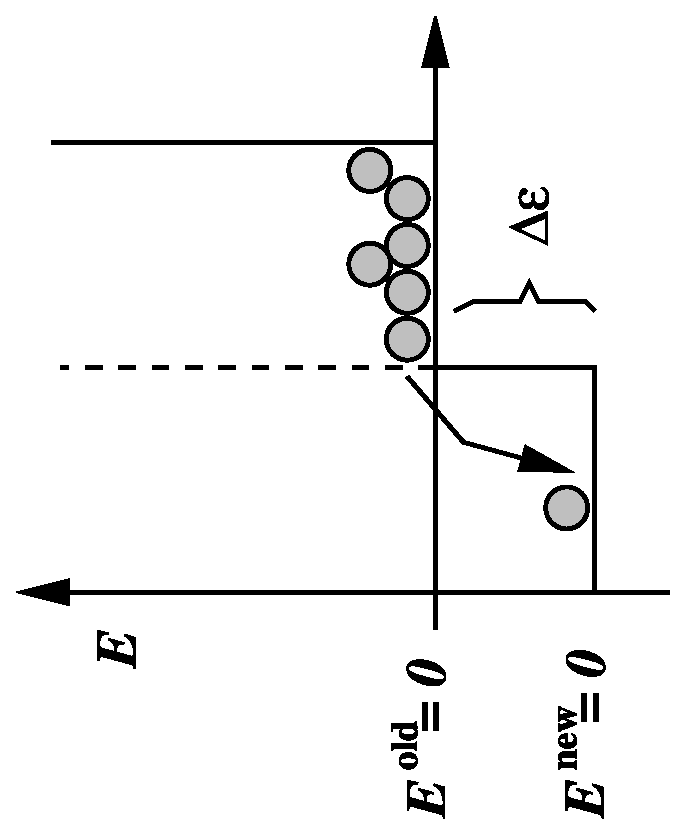
\includegraphics[width=2.1in,angle=-90]{fig1.eps}
\caption{``Energies'' (inferiorities) of strings in a first-order
  phase transition with latent heat $\Delta\epsilon$.}
\label{fig1}
\end{center}
\end{figure}

This bubble expands with a speed given by the Fisher velocity
\begin{eqnarray}
v\sim\sqrt{D\Delta\epsilon}\;, \label{eq4}
\end{eqnarray}
where $D$ is the diffusion coefficient (of information) in this
medium, until the entire population has been converted \citep{CHU}.
This marks the end of the phase transition, as the population returns
to equilibrium via mutations acting on the new species, creating new
diversity and restoring the {\em entropy} of the population to its
previous value. This prepares the stage for a new avalanche, as only
an equilibrated population is vulnerable to even the smallest
perturbation. The system has returned to a critical point, driven by
mutations, self-organized by information.

Thus we see how a first-order scenario, without coevolution, can lead
to self-organized and critical dynamics. It takes place within a
single, finite, ecological niche, and thus does not contradict the
dynamics taking place for populations that span many niches. Rather,
we must conclude that the descriptions complement each other, from the
single-niche level to the ecological web. Let us now take a closer
look at the statistics of avalanches in this model, i.e., at the
distribution of genotype sizes.


\section{Exponents and Power Laws}

\hyphenation{ap-proximated}

In this particular system avalanche size can be approximated
by the size $s$ of the genotype that gave rise to it,
Eq.~(\ref{size}).  We shall measure the distribution of these sizes
$P(s)$ in the Artificial Life system Avida, which implements a
population of self-replicating computer programs written in a simple
machine language-like instruction set of ${\cal D}=24$ instructions,
with programs of varying sequence length. In the course of
self-replication, these programs produce mutant off-spring because the
{\tt copy} instruction they use is flawed at a rate $R$ errors per
instruction copied, and adapt to an environment in which the
performance of {\em logical} computations on externally provided
numbers is akin to the catalysis of chemical reactions \citep{OBA}. In
this {\em artificial chemistry} therefore, successful computations
accelerate the metabolism (i.e., the CPU) of those strings that carry
the {\em gene} (code) necessary to perform the trick, and any program
discovering a new trick is the seed of another avalanche.

Avida is not a stirred-reactor environment (although one can be
simulated). Rather, the programs live on a two-dimensional grid, each
program occupying one site. The size of the grid is finite, and chosen
in these experiments to be small enough that avalanches are generally
over before a new one starts. As is well-known, this is the condition
{\em sine qua non} for the observation of SOC behavior, a separation
of time scales which implies that the system is driven at
infinitesimal rates.

Let $\tau$ denote the average duration of an avalanche. Then, a
separation of time scales occurs if the average time between the
production of new seeds of avalanches is much larger than $\tau$. New
seeds, in turn, are produced with a frequency $\langle\epsilon\rangle
P$, where $\langle\epsilon\rangle$ is again the average replication
rate, and $P$ is the mutation probability (per replication period) for
an average sequence of length $\ell$,
\begin{eqnarray}
P=1-(1-R)^\ell\;.
\end{eqnarray}
For small enough $R$ and not too large $\ell$ (so that the product
$R\ell$ is smaller than unity) we can approximate
$P\approx R\ell$, and infinitesimal driving occurs in the limit
\begin{eqnarray}
\langle \epsilon\rangle R\ell \ll\frac1\tau\;.\label{cond}
\end{eqnarray}
Furthermore
\begin{eqnarray}
\tau\sim\frac{L}v
\end{eqnarray}
with $L$ the diameter of the system and $v$ a typical Fisher velocity.
The fastest waves are those for which the latent heat is of the order
of the new fitness, i.e., $\Delta\epsilon\sim\epsilon$, in which case
$v\approx \epsilon$ \citep[because $D\sim\epsilon$ in
Eq.~(\ref{eq4}),][]{CHU}, and a separation of time scales is assured
whenever
\begin{eqnarray}
\frac1{R\ell}\gg {L}\;,
\end{eqnarray}
that is, in the limit of vanishing mutation rate or small population
sizes. For the $L=60$ system used here, this condition is obeyed (for
the fastest waves) only for the smallest mutation rate tested and
sequence lengths of the order of the ancestor.


\begin{figure}[t]
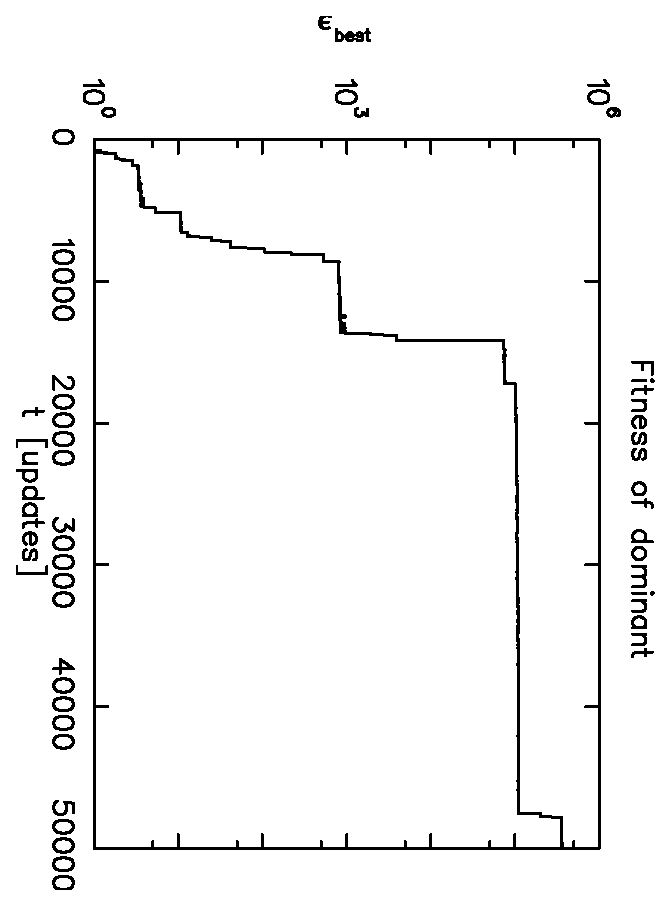
\includegraphics[width=2.3in, angle=90]{fig2.eps}
\caption{Fitness of the dominant genotype in the population, $\epsilon_{\rm best}$ as a function of time (in updates).}
\label{fig2}
\end{figure}


In the following, we keep the population size constant (a $60\times60$
grid) and vary the mutation rate. From the previous arguments, we
expect true scale-free dynamics only to appear in the limit of small
mutation rates.  As in this limit avalanches occur less and less
frequently, this is also the limit where data are increasingly
difficult to obtain, and other finite size effects can come into play.
We shall try to isolate the scale-free regime by fitting the
distribution to a power law
\begin{eqnarray}
P(s)\sim s^{-D(R)}\label{power}
\end{eqnarray}
and monitor the behavior of $D$ from low to high mutation rates.

In Fig.~\ref{fig2}, we display a typical history of $\epsilon_{\rm
best}$, i.e., the fitness of the dominant genotype.\footnote{As the
replication rate $\epsilon$ is exponential in the bonus obtained for a
successful computation, $\epsilon_{\rm best}$ increases exponentially
with time.}  Note the ``staircase'' structure of the curve reflecting
the ``punctuated'' dynamics, where each step reflects a new avalanche
and concurrently an extinction event. Staircases very much like these
are also observed in adapting populations of {\it E. Coli}
\citep{LT94}.

As touched upon earlier, the Avida world represents an environment
replete with information, which we encode by providing bonuses for
performing logical computations on externally provided (random)
numbers. The computations rewarded usually involve two inputs $A$ and
$B$, are finite in number and listed in Table~1. At the end of a
typical run (such as Fig.~\ref{fig2}) the population of programs is
usually proficient in almost all tasks for which bonuses are given
out, and the genome length has grown to several multiples of the
initial size to accommodate the acquired information.

\begin{table}[h]
\center{
\begin{tabular}{|c|c|c|c|}\hline
Name & Result & Bonus $b_i$ & Difficulty\\ \hline\hline
Echo & I/O   & 1 & --\\
Not  & $\neg A$ & 2 & 1 \\
Nand & $\neg(A\wedge B)$ & 2 & 1 \\
Not Or & $\neg A \vee B$ & 3 & 2 \\
And  &  $ A \wedge B $   & 3 & 2 \\
Or   &  $ A \vee B $     & 4 & 3 \\
And Not & $A\wedge\neg B$& 4 & 3 \\
Nor  & $\neg(A\vee B)$   & 5 & 4 \\
Xor  & $ A\ {\rm xor}\ B$ &   6 & 4 \\
Equals &$\neg(A\ {\rm xor}\ B)$&6& 4 \\ \hline
\end{tabular}
}
\vskip 0.25cm
\caption{Logical calculations on random inputs $A$ and $B$ rewarded,
bonuses, and difficulty (in minimum number of {\tt nand} instructions
required). Bonuses $b_i$ increase the speed of a CPU by a factor
$\nu_i=1+2^{b_i-3}$.}
\end{table}

Because the amount of information stored in the landscape is finite,
adaptation, and the associated avalanches, must stop when the
population has exhausted the landscape.  However, we shall see that
even a `flat' landscape (on which evolution is essentially neutral
after the sequence has optimized its replicative strategy) gives rise
to a power law of genotype sizes, as long as the programs do not
harbor an excessive amount of ``junk'' instructions.  A typical
abundance distribution (for the run depicted in Fig.~\ref{fig2}) is
shown in Fig.~\ref{fig3}.


\begin{figure}[ht]
\begin{center}
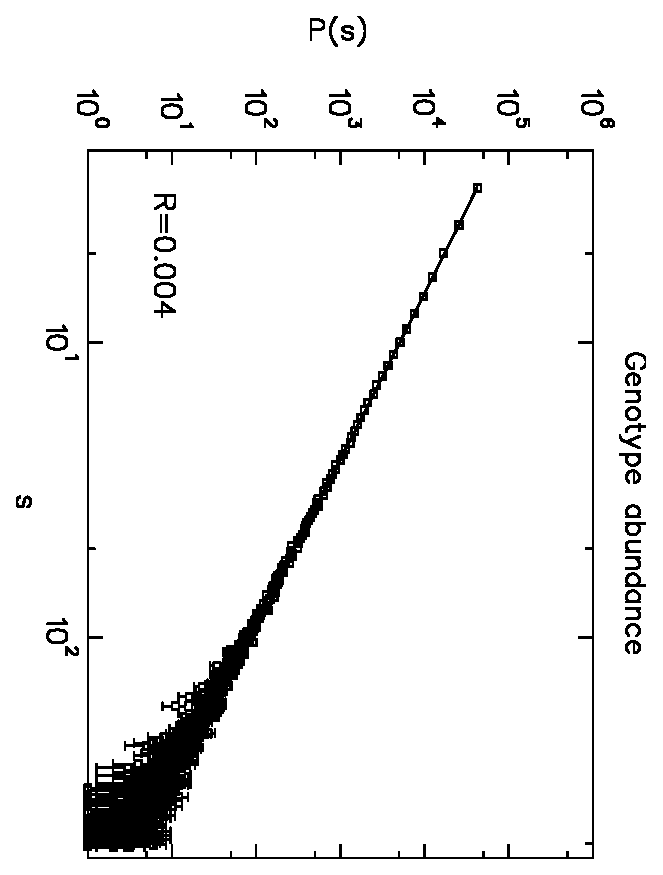
\includegraphics[width=2.25in, angle=90]{fig3.eps}
\caption{Distribution of genotypes sizes $P(s)$ fitted to a power law
  (solid line) at mutation rate $R=0.004$.}
\label{fig3}
\end{center}
\end{figure}


As mentioned earlier, we can also turn {\em off} all bonuses listed in
Tab.~1, in which case fitness is related to replicative abilities
only. Still, avalanches occur (within the first 50,000 updates
monitored) due to minute improvements in fitness, but the length of
the genomes typically stays in the range of the ancestor, a program of
length 31 instructions. We expect a change of dynamics once the
``true'' maximum of the local fitness landscape is reached, however,
we did not reach this regime in the experiments presented here. The
distribution of genotype sizes for the flat landscape is depicted in
Fig.~\ref{fig4}.


\begin{figure}[!tbp]
\begin{center}
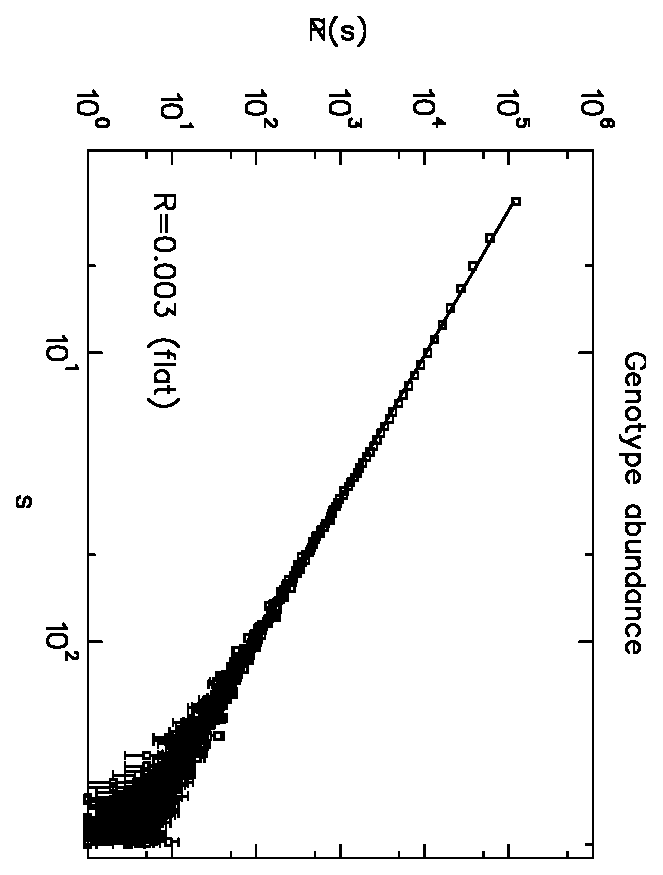
\includegraphics[width=2.25in, angle=90]{fig4.eps}
\caption{Distribution of genotypes sizes $P(s)$ for a landscape devoid
  of the bonuses listed in Tab.~1, at mutation rate $R=0.003$.} \label{fig4}
\end{center}
\end{figure}


Clearly then, even such landscapes (flat with respect to all other
activities except replication) are not neutral. Indeed, it is known
that neutral evolution, where the chance for a genotype to increase or
decrease in number is even, leads to a power law in the abundance
distribution with exponent $D=1.5$ \citep{ABH}.


\begin{figure}[t]
\begin{center}
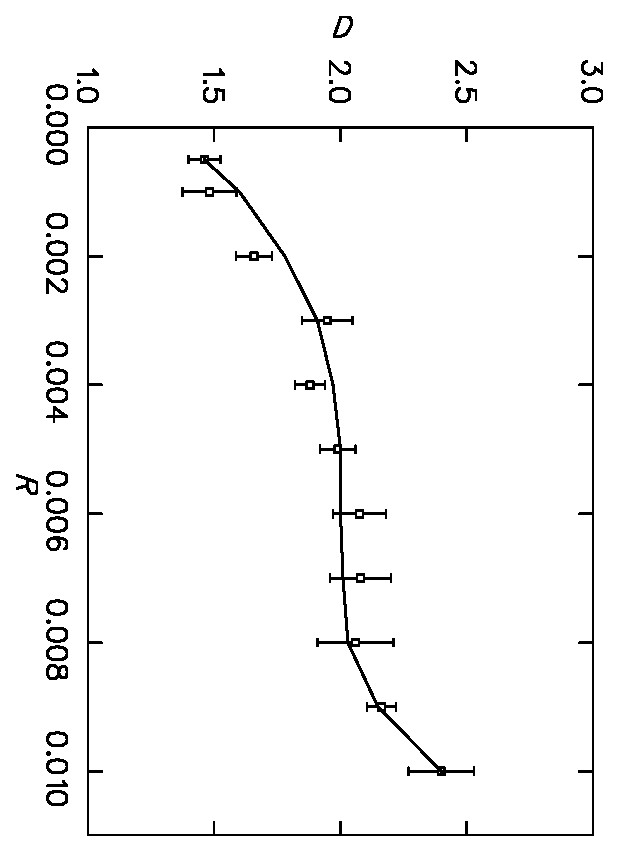
\includegraphics[width=2.2in, angle=90]{fig5.eps}
\vskip 0.25cm
\caption{Fitted exponent of power law for 34 runs at mutation rates
  between $R=0.0005$ and $R=0.01$ copy errors per instruction
  copied. The error bars reflect the standard deviation across the
  sample of runs taken at each mutation rate. The solid line is to
  guide the eye only.
}
\label{fig5}
\end{center}
\end{figure}


In order to test the dependence of the fitted exponent $D(R)$
[Eq.~(\ref{power})] on the mutation rate, we conduct a set of
experiments at varying copy-mutation rates from $0.5\times10^{-3}$ to
$10\times10^{-3}$ and take data for 50,000 updates. Again, a ``best''
genotype is not reached after this time, and we must assume that
avalanches were still occurring at the end of these runs. Furthermore,
in some runs we find that a genotype comes to dominate the population
(usually after most `genes' have been discovered) which carries an
unusual amount of junk instructions. As mentioned earlier, such
species produce a distribution that is exponentially suppressed at
large genotype sizes (data not shown). To avoid contamination from
such species, we stop recording genotypes after a plateau of fitness
was reached, i.e., if the population had discovered most of the
bonuses. Furthermore, in order to minimize finite size effects on the
determination of the critical exponent, we excluded from this fit all
genotype abundances larger than 15, i.e., we only fitted the smallest
abundances. Indeed, at larger mutation rates the higher abundances are
contaminated by a pile-up effect due to the toroidal geometry, while
at lower mutation rates a scale appears to enter which prevents
scale-free behavior. We have not, as yet, been able to determine the
origin of this scale.

In the results reported here, we show the dependence of the fitted
exponent $D$ as a function of the mutation rate $R$ used in the run,
which, however, is a good measure of the mutation probability $P$ only
at small $R$ and if the sequence length is not excessive. As a
consequence, data points at large $R$, as well as runs where an
excessive sequence length developed, carry a systematic error.

\section{Acknowledgements}

This work was supported by NSF grant No.\ PHY-9723972.

\footnotesize
\bibliographystyle{apalike}
\bibliography{example} % replace by the name of your .bib file


\end{document}
